\documentclass[border=4pt,varwidth=6in]{standalone}
\usepackage[T1]{fontenc}
\usepackage{mathptmx}
\usepackage[scaled=0.92]{helvet}
\usepackage{courier}
\usepackage{setspace}
\usepackage{amsmath,amssymb,amsthm}
\usepackage{xcolor}
\usepackage{graphicx}
\usepackage{float}
\usepackage[font={singlespacing,normalsize},labelfont=bf,labelsep=period,justification=justified,singlelinecheck=false]{caption}
\usepackage{subcaption}
\usepackage{booktabs,multirow,longtable,threeparttable,array,tabularx}
\usepackage{enumitem}
%% preamble.tex — packages and macros shared by all chapters
% Engine compatibility: biber writes UTF-8 into the .bbl. Under pdfTeX, inputenc maps
% characters outside Latin-1 to T1 glyphs; under XeTeX (tectonic) they would be silently
% dropped from the 8-bit Times fonts, so map them explicitly.
\usepackage{iftex}
\ifXeTeX
  \usepackage{newunicodechar}
  \newunicodechar{č}{\v{c}}\newunicodechar{Č}{\v{C}}\newunicodechar{ě}{\v{e}}\newunicodechar{ř}{\v{r}}
  \newunicodechar{š}{\v{s}}\newunicodechar{Š}{\v{S}}\newunicodechar{ž}{\v{z}}\newunicodechar{Ž}{\v{Z}}
  \newunicodechar{Ł}{\L{}}\newunicodechar{ł}{\l{}}\newunicodechar{ń}{\'n}\newunicodechar{ś}{\'s}
  \newunicodechar{ć}{\'c}\newunicodechar{ż}{\.z}\newunicodechar{ź}{\'z}\newunicodechar{ę}{\k{e}}\newunicodechar{ą}{\k{a}}
  \newunicodechar{ő}{\H{o}}\newunicodechar{ű}{\H{u}}\newunicodechar{ğ}{\u{g}}\newunicodechar{ş}{\c{s}}\newunicodechar{ı}{\i}
\fi
\usepackage{physics}          % \ket, \bra, \expval, \dd, \abs, \norm
\usepackage{bm}
\usepackage{mathtools}
\usepackage{siunitx}
\sisetup{detect-all,per-mode=symbol,range-phrase=--,range-units=single}
\usepackage{tikz}
\usetikzlibrary{quantikz2}
\usetikzlibrary{arrows.meta,positioning,calc,shapes.geometric,fit,backgrounds,matrix,decorations.pathreplacing}
\usepackage{pgfplots}
\pgfplotsset{compat=1.18}
\usepgfplotslibrary{groupplots,fillbetween}
\usepackage[ruled,vlined,linesnumbered]{algorithm2e}
\SetAlFnt{\singlespacing\small}
% cleveref is loaded by ttuthesis.cls *before* algorithm2e, so its algorithm2e alias is never
% installed; name the algocf label type explicitly so \cref{alg:...} prints "Algorithm N".
\usepackage{listings}
\lstset{basicstyle=\ttfamily\footnotesize\singlespacing,breaklines=true,columns=fullflexible,
        keepspaces=true,frame=single,framerule=0.3pt,xleftmargin=1em,showstringspaces=false,
        commentstyle=\itshape\color{black!60},keywordstyle=\bfseries}
\lstdefinelanguage{qasm}{morekeywords={OPENQASM,include,qubit,bit,h,cx,rz,ry,measure,reset,barrier},sensitive=true,morecomment=[l]{//}}

% Theorem-like environments (numbered per chapter, Arabic chapter number)

% Color-blind-safe palette for plots (also varies markers/line styles: TTU accessibility rule)
\definecolor{cbBlue}{HTML}{0072B2}
\definecolor{cbOrange}{HTML}{E69F00}
\definecolor{cbGreen}{HTML}{009E73}
\definecolor{cbRed}{HTML}{D55E00}
\definecolor{cbPurple}{HTML}{CC79A7}
\definecolor{cbSky}{HTML}{56B4E9}
\definecolor{cbGray}{HTML}{555555}
\pgfplotscreateplotcyclelist{ttu}{%
  {cbBlue,mark=*,solid},{cbOrange,mark=square*,dashed},{cbGreen,mark=triangle*,dotted},
  {cbRed,mark=diamond*,dashdotted},{cbPurple,mark=pentagon*,densely dashed},{cbGray,mark=o,loosely dotted}}
\pgfplotsset{every axis/.append style={cycle list name=ttu,width=0.8\linewidth,height=0.5\linewidth,
  tick label style={font=\small},label style={font=\small},legend style={font=\footnotesize,cells={anchor=west}},
  grid=major,grid style={black!12}}}

% Domain macros
\newcommand{\qgear}{Q-GEAR}
\newcommand{\deal}{DEAL}
\newcommand{\qawa}{QAWA}
\newcommand{\qpie}{QPIE}
\newcommand{\vqt}{VQT}
\newcommand{\shardq}{ShardQ}
\newcommand{\nnqa}{NNQA}
\newcommand{\rubriq}{RubriQ}
\newcommand{\cudaq}{CUDA-Q}
\newcommand{\qiskit}{Qiskit}
\newcommand{\qcrank}{QCrank}
\newcommand{\bigO}[1]{\mathcal{O}\!\left(#1\right)}
\newcommand{\Hcost}{H_C}
\newcommand{\Hmix}{H_M}
\newcommand{\code}[3]{[[#1,#2,#3]]}
\newcommand{\eps}{\varepsilon}
\newcommand{\R}{\mathbb{R}}
\newcommand{\C}{\mathbb{C}}
\newcommand{\Z}{\mathbb{Z}}
% \Tr provided by physics
\DeclareMathOperator{\poly}{poly}
\DeclareMathOperator*{\argmin}{arg\,min}
\DeclareMathOperator*{\argmax}{arg\,max}

\newcommand{\todo}[1]{{\color{red!70!black}\textbf{[TODO: #1]}}}
\providecommand{\cref}[1]{#1}
\providecommand{\Cref}[1]{#1}
\providecommand{\labelcref}[1]{#1}
\providecommand{\ref}[1]{#1}
\providecommand{\cite}[1]{[#1]}
\begin{document}
\begin{figure}[H]
\centering
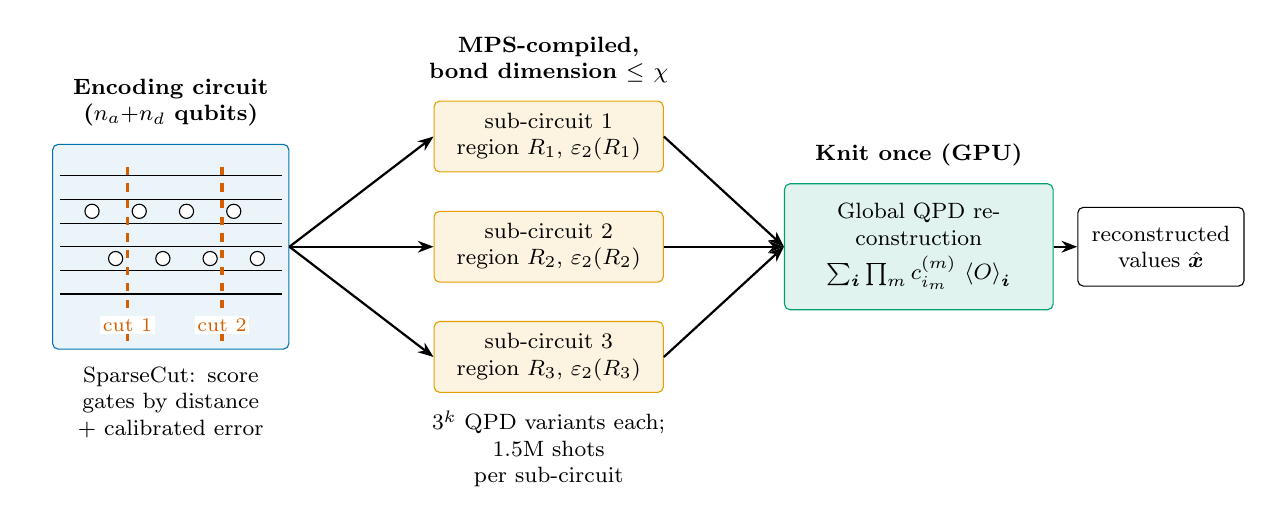
\begin{tikzpicture}[
  font=\footnotesize,
  box/.style={draw,rounded corners=2pt,align=center,inner sep=3pt},
  arr/.style={-{Stealth[length=2mm]},thick},
  node distance=6mm]
\node[box,minimum width=30mm,minimum height=26mm,fill=cbBlue!8,draw=cbBlue] (full) at (0,0) {};
\node[above=1mm of full.north,font=\footnotesize\bfseries,align=center,text width=34mm] {Encoding circuit\\($n_a{+}n_d$ qubits)};
\foreach \y in {9,6,3,0,-3,-6} {\draw ($(full.west)+(1mm,\y mm)$) -- ($(full.east)+(-1mm,\y mm)$);}
\foreach \x in {-10,-4,2,8} {\draw[fill=white] ($(full.center)+(\x mm,4.5mm)$) circle (0.9mm);}
\foreach \x in {-7,-1,5,11} {\draw[fill=white] ($(full.center)+(\x mm,-1.5mm)$) circle (0.9mm);}
\draw[cbRed,dashed,very thick] ($(full.center)+(-5.5mm,-12mm)$) -- ($(full.center)+(-5.5mm,11mm)$);
\draw[cbRed,dashed,very thick] ($(full.center)+(6.5mm,-12mm)$) -- ($(full.center)+(6.5mm,11mm)$);
\node[cbRed,font=\scriptsize] at ($(full.center)+(-5.5mm,-10mm)$) [fill=white,inner sep=1pt] {cut 1};
\node[cbRed,font=\scriptsize] at ($(full.center)+(6.5mm,-10mm)$) [fill=white,inner sep=1pt] {cut 2};
\node[below=1mm of full.south,text width=34mm,align=center] {SparseCut: score gates by distance $+$ calibrated error};
\node[box,fill=cbOrange!12,draw=cbOrange,text width=27mm,minimum height=9mm] (s1) at (4.8,1.4) {sub-circuit 1\\region $R_1$, $\eps_2(R_1)$};
\node[box,fill=cbOrange!12,draw=cbOrange,text width=27mm,minimum height=9mm] (s2) at (4.8,0.0) {sub-circuit 2\\region $R_2$, $\eps_2(R_2)$};
\node[box,fill=cbOrange!12,draw=cbOrange,text width=27mm,minimum height=9mm] (s3) at (4.8,-1.4) {sub-circuit 3\\region $R_3$, $\eps_2(R_3)$};
\node[above=1mm of s1.north,font=\footnotesize\bfseries,align=center,text width=36mm] {MPS-compiled,\\bond dimension $\le\chi$};
\node[below=1mm of s3.south,text width=32mm,align=center] {$3^{k}$ QPD variants each;\\$1.5$M shots per sub-circuit};
\node[box,fill=cbGreen!12,draw=cbGreen,text width=32mm,minimum height=16mm] (rec) at (9.5,0) {Global QPD reconstruction\\[3pt]$\sum_{\bm{i}}\prod_{m} c^{(m)}_{i_m}\,\expval{O}_{\bm{i}}$};
\node[above=1mm of rec.north,font=\footnotesize\bfseries] {Knit once (GPU)};
\node[box,right=3mm of rec,text width=19mm,minimum height=10mm] (out) {reconstructed\\values $\hat{\bm{x}}$};
\draw[arr] (full.east) -- (s1.west);
\draw[arr] (full.east) -- (s2.west);
\draw[arr] (full.east) -- (s3.west);
\draw[arr] (s1.east) -- (rec.west);
\draw[arr] (s2.east) -- (rec.west);
\draw[arr] (s3.east) -- (rec.west);
\draw[arr] (rec) -- (out);
\end{tikzpicture}
\end{figure}
\end{document}
